%%%%%%%%%%%%%%%%%%%%%%%%%%%%%%%%%%%%%%%%%%%%%%%%%%%%%%%%%%%%%%%%%%%%%%%%
%                                                                      %
%     File: Introduction/01_Motivation.tex                             %
%     Tex Master: ../Thesis.tex                                        %
%                                                                      %
%%%%%%%%%%%%%%%%%%%%%%%%%%%%%%%%%%%%%%%%%%%%%%%%%%%%%%%%%%%%%%%%%%%%%%%%

% ==============================================================================
\section{Motivation}
\label{sec:intro_motivation}

% Why does maritime awareness matter?
Saving lives at sea, protecting marine ecosystems, and securing maritime infrastructure all rely on knowing what is happening, where, and when. In vast and changing maritime environments, this requires reliable and detailed awareness over long periods. The \gls{emsa} recognises this need and highlights continuous monitoring and locally persistent operations as the basis of effective maritime surveillance and response~\cite{europeanmaritimesafetyagencyEMSAOutlook2025_v302025}.

% Which assets provide it, and what limits them?
Surface vessels provide a physical presence at sea, with long endurance and a large payload capacity~\cite{introduction_motivation_vessel_sensors,introduction_motivation_vessel_tasks}, but they only see as far as the horizon, and operating them is expensive~\cite{introduction_motivation_vessel_limitations}. Aerial platforms, such as manned aircraft and \glspl{uav}, deploy quickly and sense from above~\cite{introduction_motivation_aerial_surveillance}. Aircraft are costly, however, and \glspl{uav} suffer from short endurance and unreliable communication~\cite{introduction_motivation_uavs_limitations}.

% Why make them work together?
Each of these assets compensates for what the other lacks. \glspl{usv} keep a presence at sea for long periods at a much lower cost than crewed vessels, and \glspl{uav} extend their reach by sensing from the air, beyond the horizon of the vessel. Working as a team, a \gls{usv} and a \gls{uav} can therefore keep a continuous and local awareness that neither achieves alone.

% Why connect them with a tether?
A tether between the two vehicles strengthens this cooperation, since it supplies the \gls{uav} with power and a reliable communication link from the \gls{usv}~\cite{introduction_motivation_tethered_drones}. With the energy and the communication on the \gls{usv}, the two main limits of maritime \glspl{uav}, a short endurance and a weak long-range link, are overcome. Such systems already exist in industry. Exail and Elistair integrated a tethered \gls{uav} on the DriX \gls{usv} for persistent maritime surveillance~\cite{exail_elistair_tethered}, and ACUA Ocean and Teledyne FLIR Defense demonstrated a tethered aerial-surface system for long-endurance maritime security~\cite{acua_ocean_teledyne_mod}. Figure~\ref{fig:tether_scheme} illustrates the system considered in this work.

\begin{figure}[htbp]
    \centering
    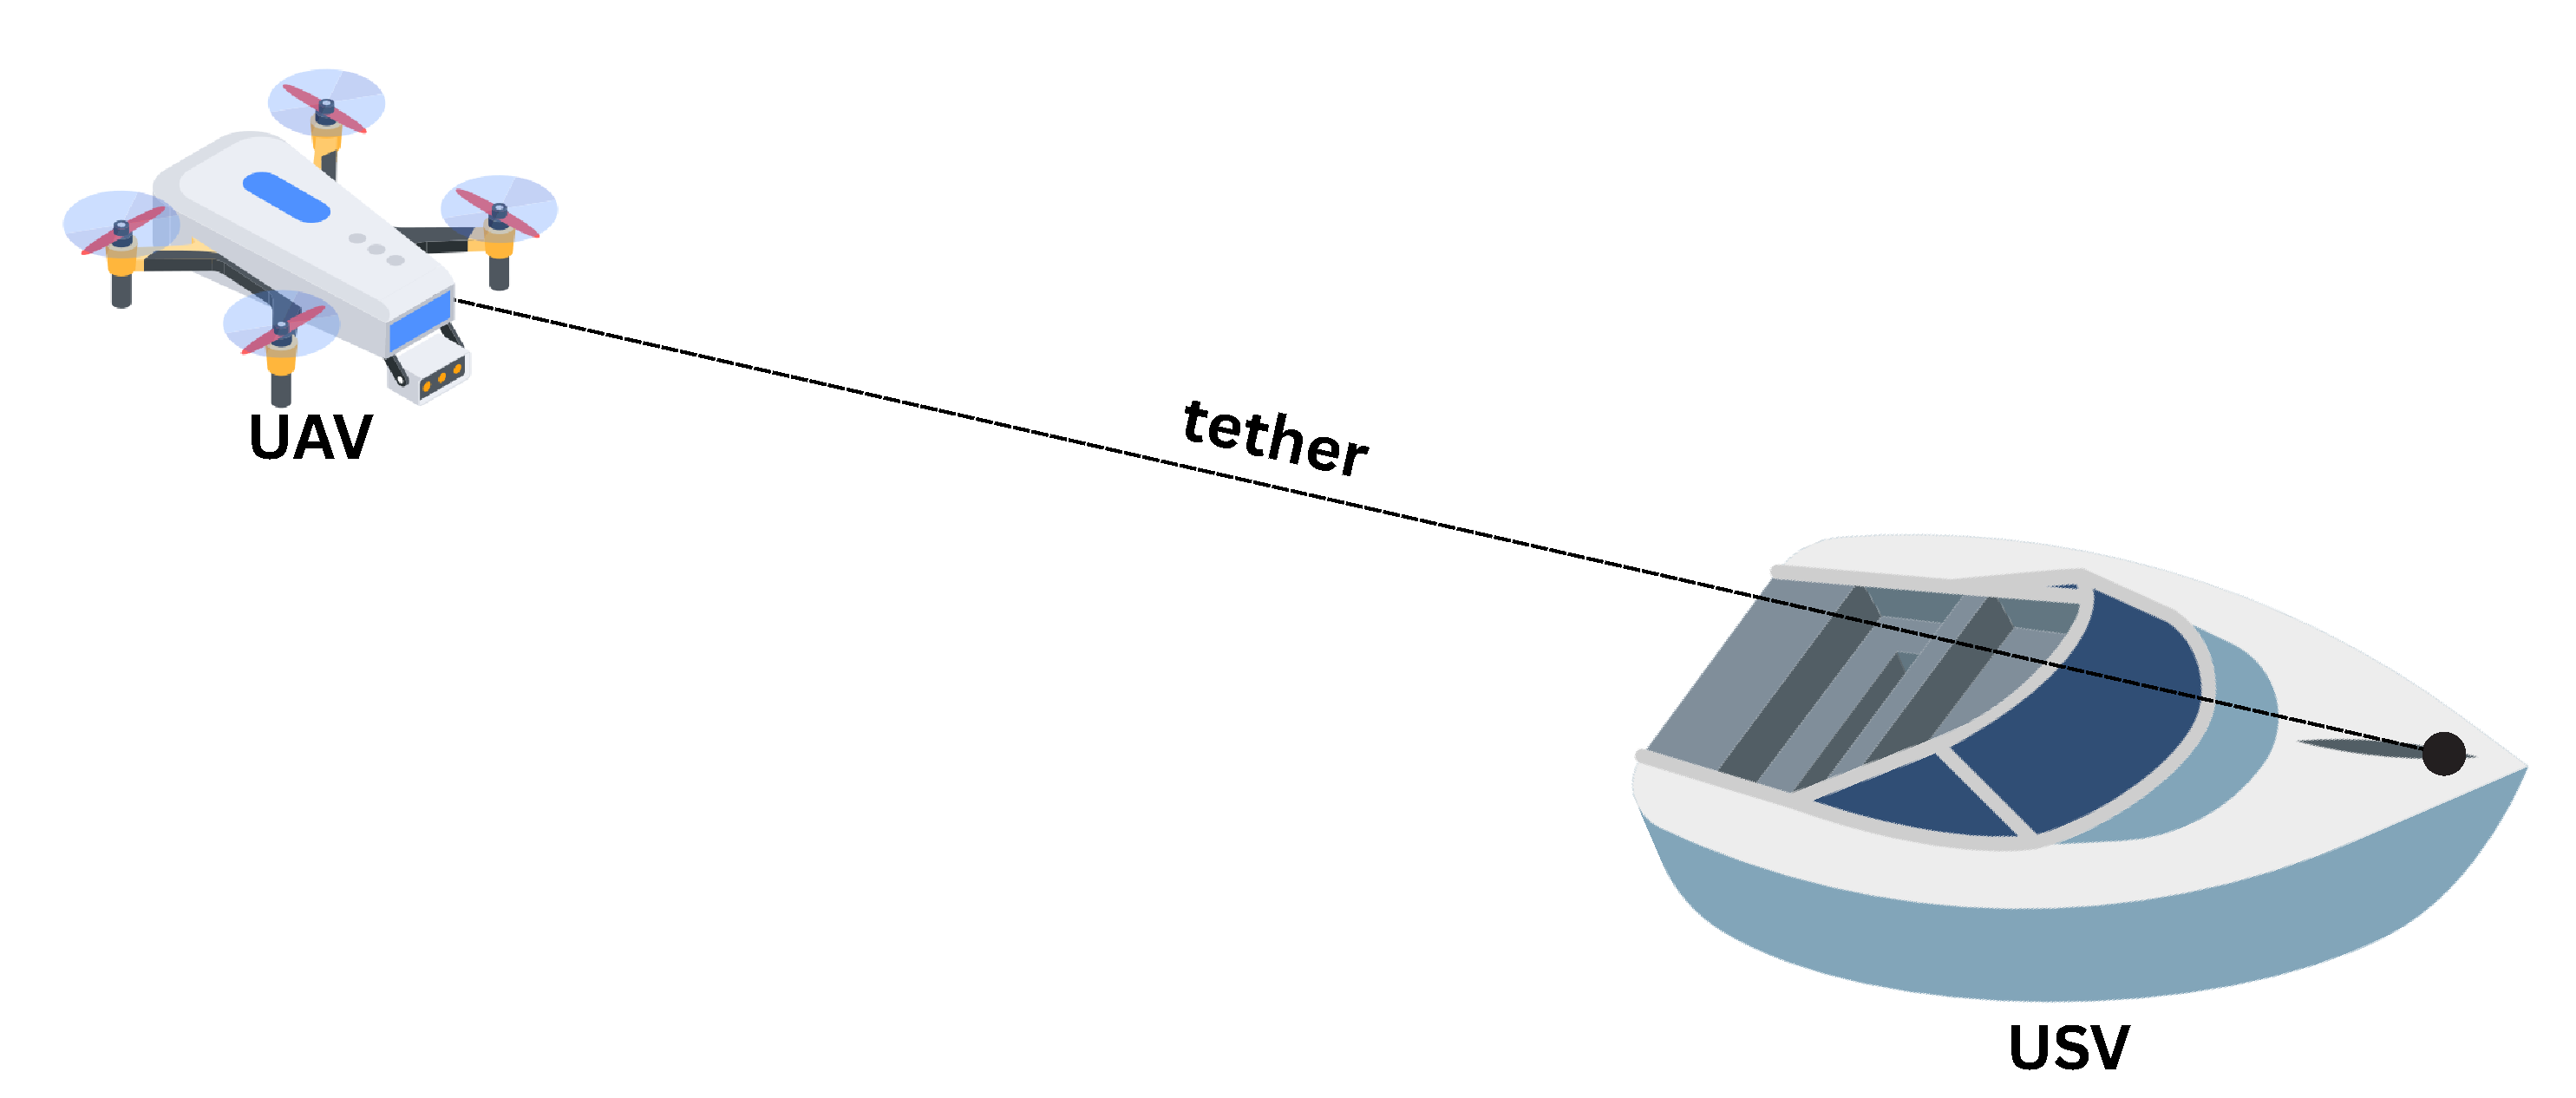
\includegraphics[width=0.65\linewidth]{Introduction/figures/system.pdf}
    \caption{Tethered \gls{usv}--\gls{uav} system.}
    \label{fig:tether_scheme}
\end{figure}

% What makes such a system hard to control?
The tether turns the two vehicles into a single system. The distance between them must stay within the reach of the tether, so the motion of one restricts the motion of the other. The two vehicles also move on very different time scales, the \gls{usv} slowly, dominated by its inertia and the drag of the water, and the \gls{uav} quickly. On top of this, wind and waves disturb both vehicles, and the \gls{uav} must take off from and land on a deck that moves with the waves.

% What is missing in existing work?
Most existing tethered \gls{uav} systems focus on the supply of power and communication, while their operation remains manual or semi-autonomous. In research, the two vehicles are often controlled separately, the tether is simplified, or the surface vessel is assumed to be fixed. These assumptions simplify the design of the controllers, but few approaches coordinate both vehicles while accounting for the tether under realistic maritime conditions.
